% quartet cheat sheet: two landscape A4 pages.  Build: make cheatsheet
% Every number here comes from lib/quartet_ctl.h and lib/quartet_voice.h
% (dial values printed from that code).
\documentclass{article}
\usepackage[a4paper,landscape,margin=6mm]{geometry}
\usepackage[T1]{fontenc}
\usepackage{lmodern}
\usepackage[default]{sourcesanspro}
\usepackage{amssymb}
\usepackage{amsmath}
\usepackage{tikz}
\usepackage[most]{tcolorbox}
\usepackage{array}
\usepackage{tabularx}
\pagestyle{empty}
\setlength{\parindent}{0pt}

\definecolor{ink}{RGB}{30,30,30}
\definecolor{snd}{RGB}{20,20,20}       % SOUND-page knob labels
\definecolor{modc}{RGB}{0,130,120}     % MOD-page knob labels
\definecolor{vcoc}{RGB}{170,90,20}     % oscillator
\definecolor{fltc}{RGB}{190,40,60}     % filters
\definecolor{egc}{RGB}{150,60,170}     % envelope
\definecolor{ensc}{RGB}{30,90,170}     % Ensemble
\definecolor{freec}{RGB}{170,170,170}  % unassigned
\definecolor{padc}{RGB}{120,170,230}

\newcommand{\MD}[1]{\textcolor{modc}{#1}}
\newcommand{\VC}[1]{\textcolor{vcoc}{#1}}
\newcommand{\FL}[1]{\textcolor{fltc}{#1}}
\newcommand{\EG}[1]{\textcolor{egc}{#1}}
\newcommand{\EN}[1]{\textcolor{ensc}{#1}}
\newcommand{\FR}[1]{\textcolor{freec}{#1}}
\newcommand{\cc}[1]{\textcolor{black!45}{\fontsize{4.6}{5}\selectfont #1}}

% knob: x, SOUND label (above), MOD label (below)
\newcommand{\knob}[3]{%
  \draw[fill=black!8, draw=black!60, line width=0.4pt] (#1,63) circle (3.4);
  \draw[black!60, line width=0.5pt] (#1,63) -- ++(110:2.9);
  \node[font=\fontsize{5.4}{6}\selectfont\bfseries, text=snd, align=center] at (#1,70.2) {#2};
  \node[font=\fontsize{5.2}{5.8}\selectfont, text=modc, align=center] at (#1,56.2) {#3};}
\newcommand{\pad}[3]{%
  \draw[rounded corners=0.8mm, fill=padc!35!white, draw=padc!80!black, line width=0.4pt]
    (36+#1*13.2, 19+#2*13.2) rectangle ++(12,12);
  \node[font=\fontsize{5.4}{6}\selectfont, text=ink, align=center, text width=11mm]
    at (36+#1*13.2+6, 19+#2*13.2+6) {#3};}
\newcommand{\fader}[3]{%
  \draw[fill=black!12, draw=black!50] (#1-0.7,26) rectangle (#1+0.7,50);
  \draw[fill=#3!60!white, draw=#3!70!black, rounded corners=0.4mm] (#1-2.6,36) rectangle (#1+2.6,40);
  \node[font=\fontsize{5.4}{6}\selectfont\bfseries, text=#3!70!black, align=center] at (#1,55) {#2};}
\newcommand{\btn}[5]{%
  \draw[rounded corners=0.6mm, fill=#4!25!white, draw=#4!70!black, line width=0.4pt]
    (#1-#5/2,#2-2.6) rectangle (#1+#5/2,#2+2.6);
  \node[font=\fontsize{4.9}{5.4}\selectfont, text=ink, align=center] at (#1,#2) {#3};}

\tcbset{card/.style={enhanced, colback=white, colframe=black!70, boxrule=0.5pt, arc=1.5mm,
    left=1.6mm, right=1.6mm, top=1.1mm, bottom=1.1mm, toptitle=0.6mm, bottomtitle=0.6mm,
    fonttitle=\bfseries\fontsize{8.6}{10}\selectfont, coltitle=white, colbacktitle=black!75,
    fontupper=\fontsize{7.1}{8.5}\selectfont, before skip=0mm, after skip=1.8mm}}
\newtcolorbox{card}[1]{card, title={#1}}
\newcolumntype{L}{>{\raggedright\arraybackslash}X}

\begin{document}

{\fontsize{16}{18}\selectfont\bfseries quartet}\hspace{3mm}%
{\fontsize{9.5}{11}\selectfont Axoloti Core + Launchkey 49 MK3 (standalone mode) \textperiodcentered{}
four voices after the Roland Jupiter-4 \textperiodcentered{} \texttt{patches/quartet/quartet\_v1.axp}}\hfill
{\fontsize{7}{8}\selectfont\color{black!55} v1.0 \textperiodcentered{} 2026-11-13 \textperiodcentered{} page 1 of 2}

\vspace{1.5mm}
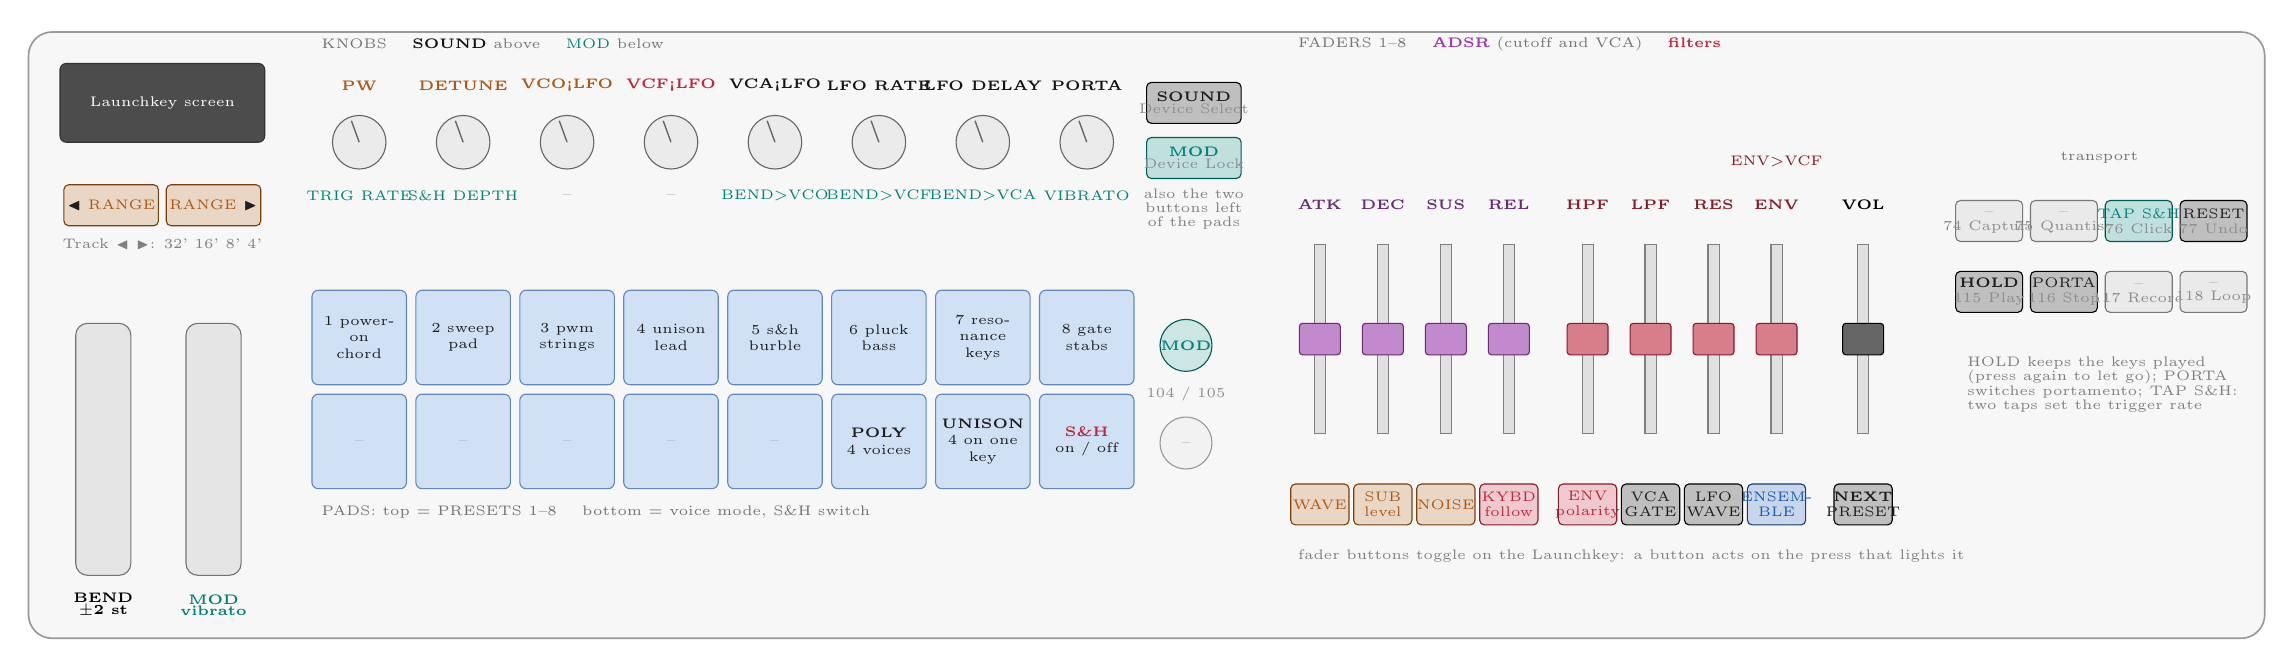
\begin{tikzpicture}[x=1mm,y=1mm]
  \draw[rounded corners=3mm, fill=black!3, draw=black!40, line width=0.6pt] (0,0) rectangle (284,77);

  % ---- left: screen, track buttons, wheels
  \draw[fill=black!70, draw=black!80, rounded corners=0.8mm] (4,63) rectangle (30,73);
  \node[font=\fontsize{5}{6}\selectfont, text=white] at (17,68) {Launchkey screen};
  \btn{10.5}{55}{\(\blacktriangleleft\) \VC{RANGE}}{vcoc}{12}
  \btn{23.5}{55}{\VC{RANGE} \(\blacktriangleright\)}{vcoc}{12}
  \node[font=\fontsize{4.6}{5}\selectfont, text=black!50] at (17,50) {Track \(\blacktriangleleft\) \(\blacktriangleright\): 32' 16' 8' 4'};
  \draw[rounded corners=1.5mm, fill=black!10, draw=black!55] (6,8) rectangle (13,40);
  \draw[rounded corners=1.5mm, fill=black!10, draw=black!55] (20,8) rectangle (27,40);
  \node[font=\fontsize{5.4}{6}\selectfont\bfseries, align=center] at (9.5,4.2) {BEND\\[-0.6mm]\(\pm\)2 st};
  \node[font=\fontsize{5.4}{6}\selectfont\bfseries, align=center, text=modc] at (23.5,4.2) {MOD\\[-0.6mm]vibrato};

  % ---- knobs: SOUND (top) / MOD (green)
  \node[font=\fontsize{5}{6}\selectfont, text=black!55, anchor=west] at (36,75.5) {KNOBS \quad
     \textbf{\textcolor{snd}{SOUND}} above \quad \MD{MOD} below};
  \knob{42}{\VC{PW}}{\MD{TRIG RATE}}
  \knob{55.2}{\VC{DETUNE}}{\MD{S\&H DEPTH}}
  \knob{68.4}{\VC{VCO<LFO}}{\FR{--}}
  \knob{81.6}{\FL{VCF<LFO}}{\FR{--}}
  \knob{94.8}{VCA<LFO}{\MD{BEND>VCO}}
  \knob{108}{LFO RATE}{\MD{BEND>VCF}}
  \knob{121.2}{LFO DELAY}{\MD{BEND>VCA}}
  \knob{134.4}{PORTA}{\MD{VIBRATO}}
  \btn{148}{68}{\textbf{SOUND}\\[-0.4mm]\cc{Device Select}}{black}{12}
  \btn{148}{61}{\textbf{\MD{MOD}}\\[-0.4mm]\cc{Device Lock}}{modc}{12}
  \node[font=\fontsize{4.4}{5}\selectfont, text=black!50, align=center] at (148,54.5) {also the two\\buttons left\\of the pads};

  % ---- pads
  \pad{0}{1}{1 power-on\\chord} \pad{1}{1}{2 sweep\\pad} \pad{2}{1}{3 pwm\\strings} \pad{3}{1}{4 unison\\lead}
  \pad{4}{1}{5 s\&h\\burble} \pad{5}{1}{6 pluck\\bass} \pad{6}{1}{7 resonance\\keys} \pad{7}{1}{8 gate\\stabs}
  \pad{0}{0}{\FR{--}} \pad{1}{0}{\FR{--}} \pad{2}{0}{\FR{--}} \pad{3}{0}{\FR{--}} \pad{4}{0}{\FR{--}}
  \pad{5}{0}{\textbf{POLY}\\4 voices} \pad{6}{0}{\textbf{UNISON}\\4 on one\\key} \pad{7}{0}{\FL{\textbf{S\&H}}\\on / off}
  \node[font=\fontsize{5}{6}\selectfont, text=black!55, anchor=west] at (36,16) {PADS: top = PRESETS 1--8 \quad bottom = voice mode, S\&H switch};
  \draw[fill=modc!20, draw=modc!70!black] (147,37.2) circle (3.3);
  \draw[fill=black!5, draw=black!40] (147,24.8) circle (3.3);
  \node[font=\fontsize{4.6}{5}\selectfont\bfseries, text=modc] at (147,37.2) {MOD};
  \node[font=\fontsize{4.6}{5}\selectfont, text=freec] at (147,24.8) {--};
  \node[font=\fontsize{4.2}{5}\selectfont, text=black!45] at (147,31) {104 / 105};

  % ---- faders: ADSR, filters, volume
  \node[font=\fontsize{5}{6}\selectfont, text=black!55, anchor=west] at (160,75.5) {FADERS 1--8 \quad
     \EG{\textbf{ADSR}} (cutoff and VCA) \quad \FL{\textbf{filters}}};
  \fader{164}{ATK}{egc} \fader{172}{DEC}{egc} \fader{180}{SUS}{egc} \fader{188}{REL}{egc}
  \fader{198}{HPF}{fltc} \fader{206}{LPF}{fltc} \fader{214}{RES}{fltc} \fader{222}{ENV}{fltc}
  \node[font=\fontsize{4.6}{5}\selectfont, text=fltc!70!black, align=center] at (222,60.5) {ENV>VCF};
  \fader{233}{VOL}{black}
  \btn{164}{17}{\VC{WAVE}}{vcoc}{7.4}
  \btn{172}{17}{\VC{SUB}\\\VC{level}}{vcoc}{7.4}
  \btn{180}{17}{\VC{NOISE}}{vcoc}{7.4}
  \btn{188}{17}{\FL{KYBD}\\\FL{follow}}{fltc}{7.4}
  \btn{198}{17}{\FL{ENV}\\\FL{polarity}}{fltc}{7.4}
  \btn{206}{17}{VCA\\GATE}{black}{7.4}
  \btn{214}{17}{LFO\\WAVE}{black}{7.4}
  \btn{222}{17}{\EN{ENSEM-}\\\EN{BLE}}{ensc}{7.4}
  \btn{233}{17}{\textbf{NEXT}\\PRESET}{black}{7.4}
  \node[font=\fontsize{4.6}{5}\selectfont, text=black!50, anchor=west] at (160,10.5) {fader buttons toggle on the Launchkey: a button acts on the press that lights it};

  % ---- transport (ch 16)
  \node[font=\fontsize{5}{6}\selectfont, text=black!55] at (263,61) {transport};
  \btn{249}{53}{\FR{--}\\\cc{74 Capture}}{freec}{8.5}
  \btn{258.5}{53}{\FR{--}\\\cc{75 Quantise}}{freec}{8.5}
  \btn{268}{53}{\MD{TAP S\&H}\\\cc{76 Click}}{modc}{8.5}
  \btn{277.5}{53}{RESET\\\cc{77 Undo}}{black}{8.5}
  \btn{249}{44}{\textbf{HOLD}\\\cc{115 Play}}{black}{8.5}
  \btn{258.5}{44}{PORTA\\\cc{116 Stop}}{black}{8.5}
  \btn{268}{44}{\FR{--}\\\cc{117 Record}}{freec}{8.5}
  \btn{277.5}{44}{\FR{--}\\\cc{118 Loop}}{freec}{8.5}
  \node[font=\fontsize{4.6}{5.2}\selectfont, text=black!50, align=left, anchor=north west] at (245,37)
     {HOLD keeps the keys played\\(press again to let go); PORTA\\switches portamento; TAP S\&H:\\two taps set the trigger rate};
\end{tikzpicture}

\vspace{1.2mm}
\begin{minipage}[t]{72mm}\vspace{0pt}
\begin{card}{Signal path (as on the Jupiter-4's panel)}
\VC{VCO} (saw, square, pulse, PWM, off) + \VC{SUB} (a square an octave down; off, low, mid, high) +
\VC{NOISE} \(\to\) \FL{HPF} \(\to\) \FL{LPF} \(\to\) VCA \(\to\) \EN{Ensemble} \(\to\) VOL, stereo out.
One \EG{ADSR} per voice moves the cutoff (ENV>VCF, either polarity) and the VCA; \textbf{VCA GATE}
gives the VCA the key instead. One LFO (sine, square, saw, inverted saw) for all voices; the
\FL{S\&H} samples noise at the trigger rate and steps the cutoff.
\end{card}
\begin{card}{The filters}
\FL{LPF}: 4-pole (24 dB/oct), resonance limited as the Jupiter-4's diodes do; past \textbf{87\,\%}
(fader 111) it \textbf{self-oscillates}, a sine at the cutoff. More resonance thins the bass, as on
the original. \FL{KYBD} follow: the cutoff follows the keys by 10, 40, 70 or 100\,\%; at 100\,\% a
self-oscillating filter plays in tune. \FL{HPF}: 1-pole, no resonance; off at the bottom.
\end{card}
\end{minipage}\hfill
\begin{minipage}[t]{70mm}\vspace{0pt}
\begin{card}{Voices (bottom pads 6, 7)}
\textbf{POLY}: four voices; a new key takes the voice released longest ago, or the oldest note.
\textbf{UNISON}: all four on the lowest held key, spread by \VC{DETUNE} (outer voices up to
\(\pm\)20 cents); a lower key takes over, releasing it slides back. PORTAMENTO glides each voice
from its own last note. Each voice drifts a little in pitch (\(\pm\)3 cents), as analog ones do.
\end{card}
\begin{card}{Oscillator (fader buttons 1--3, Track)}
\fontsize{6.8}{8.1}\selectfont
\begin{tabularx}{\linewidth}{@{}l L@{}}
\VC{\textbf{WAVE}} & saw \(\to\) square \(\to\) pulse \(\to\) PWM \(\to\) off \\
\VC{\textbf{PW}} knob & pulse: 50, 40, 20, 10\,\% (four steps); PWM: the LFO's depth; saw, square: nothing \\
\VC{\textbf{SUB}} & off \(\to\) low \(\to\) mid \(\to\) high \\
\VC{\textbf{RANGE}} & 32', 16', 8', 4' (8' = the key's pitch) \\
\end{tabularx}
\end{card}
\end{minipage}\hfill
\begin{minipage}[t]{66mm}\vspace{0pt}
\begin{card}{Modulation}
\textbf{LFO} to the pitch (VCO<LFO), the cutoff (VCF<LFO), the level (VCA<LFO, tremolo) and,
on PWM, the pulse width. \textbf{LFO DELAY}: after a fresh key (all keys up before) the LFO fades in
over that time. \FL{\textbf{S\&H}}: bottom pad 8 switches it; S\&H DEPTH (MOD knob 2) sets how
far the cutoff jumps, TRIG RATE (or TAP S\&H) how often.
\end{card}
\begin{card}{Wheels, Ensemble}
BEND: the pitch \(\pm\)BEND>VCO (2 st at power-on), and the cutoff and the level by BEND>VCF and
BEND>VCA. MOD wheel: extra vibrato up to VIBRATO (0.47 st at power-on). \EN{\textbf{ENSEMBLE}}
(fader button 8): a stereo chorus, a slow 0.6 Hz swirl (rate and depth guessed, to tune by ear).
\end{card}
\end{minipage}\hfill
\begin{minipage}[t]{68mm}\vspace{0pt}
\begin{card}{Inside}
\fontsize{6.6}{7.8}\selectfont
LPF: four trapezoidal (zero-delay) one-poles in a ladder, the resonance fed back through a soft
clip; each sample solves one scalar equation, which has exactly one root, by 2 Newton steps
(measured error \(< 6\cdot10^{-5}\)). It self-oscillates at the cutoff (within 0.1\,\%) from
feedback 4. Oscillators at 48 kHz with 4-point BLEP edges (aliasing \(-57\) dB at C4, \(-48\) dB
at C7). Envelopes per sample; pitch and cutoff every 4 samples. Code: \texttt{lib/quartet\_voice.h}.
\end{card}
\begin{card}{Load}
DSP 8.5\,\% idle, 64.5\,\% with four voices held, 72\,\% with every source, full resonance and
the Ensemble; patch RAM 19 of 44 KB.
\end{card}
\end{minipage}

%======================================================================
\newpage
{\fontsize{16}{18}\selectfont\bfseries quartet}\hspace{3mm}%
{\fontsize{9.5}{11}\selectfont presets, dial values, recipes, troubleshooting}\hfill
{\fontsize{7}{8}\selectfont\color{black!55} v1.0 \textperiodcentered{} page 2 of 2}

\vspace{1.5mm}
\begin{minipage}[t]{150mm}\vspace{0pt}
\begin{card}{Presets: top pads = 1--8; NEXT PRESET (fader button 9) steps; RESET (Undo) = 1 \quad\textmd{\fontsize{6.5}{7}\selectfont (2--8 set from the parameter meanings, not yet tuned by ear)}}
\fontsize{7.2}{8.7}\selectfont
\begin{tabularx}{\linewidth}{@{}>{\bfseries}l L@{}}
1 power-on chord & Saw through the LPF at 1.6 kHz, resonance 0.24, the envelope opens it 2.8 octaves; portamento 0.11 s. The power-on sound. \\
2 sweep pad & Saw + sub; a 1.5 s attack opens the cutoff 4 octaves from 240 Hz at resonance 0.6, a 0.3 Hz LFO moves it half an octave; long decay and release; Ensemble. \\
3 pwm strings & PWM at 0.7 Hz, 0.6 s attack, 1.2 s release, HPF at 86 Hz, LPF at 3.5 kHz; Ensemble. \\
4 unison lead & UNISON, outer voices 9 cents apart, portamento 0.2 s, vibrato 5.5 Hz fading in after 0.6 s; resonance 0.45. \\
5 s\&h burble & Saw + sub, S\&H on: 8 steps a second, up to 1.9 octaves, around a resonant 900 Hz. \\
6 pluck bass & 16', saw + sub, no sustain: the envelope opens the cutoff 5 octaves from 230 Hz, resonance 0.6. \\
7 resonance keys & Sources off, resonance 1, keyboard follow 100\,\%: the filter sings the keys (C4 about 25 cents flat: tune with LPF). \\
8 gate stabs & VCA GATE, the envelope inverted on the cutoff (it dips and opens again), resonance 0.5. \\
\end{tabularx}\\[0.3mm]
A preset sets the switches, the voice mode, both knob pages and faders 1--8; the volume stays.
After a preset a knob or fader moves its value from where it is (no jump); it catches up at the end of its travel at the latest.
\end{card}

\begin{card}{Recipes}
\fontsize{7.4}{9.0}\selectfont
\textbf{Filter as oscillator}: WAVE off, SUB off, RES past 87\,\%, KYBD 100\,\%; tune with LPF.\quad
\textbf{Burble}: S\&H on, RES at 3/4, S\&H DEPTH at half, TRIG RATE to taste (or tap it).\quad
\textbf{Fat lead}: UNISON, DETUNE at 1/3, PORTA at 1/4.\quad
\textbf{Strings}: WAVE to PWM, PW at 3/4, LFO RATE at 1/4, ATK and REL at 3/4, ENSEMBLE.\quad
\textbf{Delayed vibrato}: VCO<LFO at 1/8, LFO RATE at 3/5 (5 Hz), LFO DELAY at 1/3 (1 s).\quad
\textbf{Bass}: RANGE 16', SUB high, SUS 0, DEC at 1/2, ENV>VCF at 2/3.
\end{card}
\end{minipage}\hfill
\begin{minipage}[t]{128mm}\vspace{0pt}
\begin{card}{Where the values fall (knob or fader at \dots)}
\fontsize{7.3}{8.9}\selectfont
\setlength{\tabcolsep}{3pt}
\begin{tabular}{@{}l r r r r r@{}}
 & 0 & 1/4 & 1/2 & 3/4 & full \\ \hline
\EG{\textbf{ATTACK}} (s) & 0.0006 & 0.005 & 0.044 & 0.35 & 3 \\
\EG{\textbf{DECAY, RELEASE}} (s) & 0.014 & 0.073 & 0.38 & 1.9 & 10 \\
\FL{\textbf{HPF}} (Hz) & off & 135 & 460 & 1500 & 5000 \\
\FL{\textbf{LPF}} (Hz, at C4) & 20 & 114 & 650 & 3500 & 20000 \\
\FL{\textbf{RES}} (feedback) & 0 & 1.2 & 2.3 & 3.4 & 4.6 (self-osc. from 4) \\
\FL{\textbf{ENV>VCF}} (oct) & 0 & 1.8 & 3.5 & 5.2 & 7 \\
\VC{\textbf{PW}} (pulse width) & 50\,\% & 40\,\% & 20\,\% & 20\,\% & 10\,\% \\
\VC{\textbf{PW}} on PWM (narrowest) & 50\,\% & 39\,\% & 27\,\% & 16\,\% & 5\,\% \\
\VC{\textbf{DETUNE}} (cents, outer) & 0 & 5 & 10 & 15 & 20 \\
\VC{\textbf{VCO<LFO}} (st) & 0 & 0.76 & 3 & 6.7 & 12 \\
\FL{\textbf{VCF<LFO}} (oct) & 0 & 0.25 & 1 & 2.2 & 4 \\
\textbf{VCA<LFO} (level dips by) & 0 & 25\,\% & 50\,\% & 75\,\% & 100\,\% \\
\textbf{LFO RATE} (Hz) & 0.1 & 0.54 & 2.9 & 15 & 80 \\
\textbf{LFO DELAY, PORTA} (s) & 0 & 0.63, 0.13 & 2.5, 0.51 & 5.6, 1.1 & 10, 2 \\
\MD{\textbf{TRIG RATE}} (Hz) & 1 & 2.3 & 5.1 & 11 & 25 \\
\MD{\textbf{S\&H DEPTH}} (oct) & 0 & 0.76 & 1.5 & 2.2 & 3 \\
\MD{\textbf{BEND>VCO / VCF / VCA}} & 0 & 3 st / 0.5 oct / 3 dB & 6 / 1 / 6 & 9 / 1.5 / 9 & 12 / 2 / 12 \\
\MD{\textbf{VIBRATO}} (st, wheel up) & 0 & 0.25 & 0.5 & 0.75 & 1 \\
\end{tabular}
\end{card}

\begin{card}{Something seems wrong?}
\fontsize{7.3}{8.9}\selectfont
\textbf{Silence}: WAVE off with SUB and NOISE off (and RES below 87\,\%), LPF at the bottom, HPF at
the top, SUS 0 with a short decay, or VOL down.\quad
\textbf{A button needs two presses}: the fader buttons toggle; they act on the press that lights them.\quad
\textbf{A knob does nothing}: PW acts only on pulse and PWM, DETUNE only in UNISON, S\&H DEPTH only
with S\&H on; or the knob has not caught up yet: keep turning.\quad
\textbf{Notes that will not stop}: HOLD (Play).\quad
\textbf{Lost}: RESET (Undo).\quad
\textbf{Another patch} (on the SD card): hold both buttons left of the pads and tap a top pad: 1 freak,
2 grains, 3 groove, 4 soliton, 5 aeolian, 6 raw, 7 quartet.
\end{card}
\end{minipage}

\end{document}
